\documentclass{article}
\usepackage{ctex}
\usepackage[xcolor]{listings} % 导入代码高亮包
\usepackage{xcolor} % 导入颜色包
\usepackage{graphicx} % 导入图形包
\usepackage[margin=1in]{geometry} % 调整页边距
\author{陈祎伟\\3230102357}
\title{Lab 3 : 动态分支预测}
\date{2025年4月9日}

\lstset{
    basicstyle=\ttfamily\footnotesize, % 基本样式,小号等宽字体
    numbers=left,                      % 行号位置
    numberstyle=\tiny\color{gray},     % 行号样式
    stepnumber=1,                      % 行号步长
    numbersep=5pt,                     % 行号与代码间距
    backgroundcolor=\color{white},     % 代码背景色
    showspaces=false,                  % 显示空格
    showstringspaces=false,            % 显示字符串中的空格
    showtabs=false,                    % 显示制表符
    frame=single,                      % 代码框
    rulecolor=\color{black},           % 框颜色
    tabsize=4,                         % 制表符宽度
    captionpos=b,                      % 标题位置
    breaklines=true,                   % 自动换行
    breakatwhitespace=false,           % 仅在空格处换行
    title=\lstname,                    % 显示文件名
    keywordstyle=\color{blue},         % 关键字颜色
    commentstyle=\color{brown},        % 注释颜色
    stringstyle=\color{red},           % 字符串颜色
    escapeinside={\%*}{*)},            % 特殊字符
    morekeywords={*,...},              % 额外关键字
    language=[x86masm]Assembler        % 定义asm语言
}

\begin{document}
\maketitle
\section{设计思路}
\subsection{BHT模块}
BHT 模块用于存储历史跳转信息。\par
在 BHT 的实现中,我使用了类似哈希表的方式来存储跳转信息。BHT 的大小为 256,使用 8 位索引来访问。\par
具体实现如下:\par
\begin{enumerate}
    \item 模块接口定义以及初始化:\par
    \begin{itemize}
        \item 模块接口定义如下:\par
        \begin{lstlisting}[language=Verilog]
    module BHT(
        input clk,
        input rst,
        input [31:0] PC_IF,
        input bht_wen,
        input taken,
        output wire bht_pridict
        );
        \end{lstlisting}
        其中,PC\_IF 为当前指令地址,bht\_wen 为写使能信号,taken 为 ID 阶段真实跳转结果,bht\_pridict 为预测结果。\par

        \item 定义参数如下:\par
        \begin{lstlisting}[language=Verilog]
    parameter Pridict_Strongly_Taken = 2'b11;
    parameter Pridict_Weakly_Taken = 2'b10;
    parameter Pridict_Weakly_Not_Taken = 2'b01;
    parameter Pridict_Strongly_Not_Taken = 2'b00;

    parameter BHT_SIZE = 256; // Number of entries in the BHT
    \end{lstlisting}
        同时,将 BHT 各项的初始值设置为 Pridict\_Weakly\_Not\_Taken。\par

    \end{itemize}

    \item 输出预测结果 bht\_pridict 的实现:\par
    \begin{lstlisting}[language=Verilog]
    assign bht_pridict = bht[PC_IF[9:2]] >= Pridict_Weakly_Taken;
    \end{lstlisting}
    这里将 PC\_IF / 4 ,即指令数,取低 8 位作为 BHT 的索引。\par
    当 bht 中的值大于等于 Pridict\_Weakly\_Taken 时,即给出预测值 1, 否则为 0。\par

    \item BHT 的更新:\par
    由于 BHT 是基于 PC\_IF 的预测,这里使用 reg 将 PC\_IF 进行存储。\par
    \begin{lstlisting}[language=Verilog]
    reg [31:0] PC_IF_reg;
    initial begin
        PC_IF_reg = 32'b0; // Initialize the PC_IF register
    end
    always @(posedge clk or posedge rst) begin
        if (rst) begin
            PC_IF_reg <= 32'b0; // Reset the PC_IF register
        end else begin
            PC_IF_reg <= PC_IF; // Update the PC_IF register
        end
    end
    \end{lstlisting}

    在接收到 bht\_wen 信号时,根据 PC\_IF\_reg 和实际跳转情况 taken, 更新 BHT 的值:\par
    \begin{lstlisting}[language=Verilog]
    always @(posedge clk or posedge rst) begin
        if (rst) begin
            for (i = 0; i < BHT_SIZE; i = i + 1) begin
                bht[i] <= Pridict_Weakly_Not_Taken; // Reset all entries to Weakly Not Taken
            end
        end else begin
            if (bht_wen) begin
                if (taken) begin
                    bht[PC_IF_reg[9:2]] <= (bht[PC_IF_reg[9:2]] == Pridict_Strongly_Taken) ? Pridict_Strongly_Taken : bht[PC_IF_reg[9:2]] + 1; // Increment if taken
                end else begin
                    bht[PC_IF_reg[9:2]] <= (bht[PC_IF_reg[9:2]] == Pridict_Strongly_Not_Taken) ? Pridict_Strongly_Not_Taken : bht[PC_IF_reg[9:2]] - 1; // Decrement if not taken
                end
            end
        end
    end
    \end{lstlisting}
\end{enumerate}

\subsection{BTB 模块}
BTB 模块用于存储跳转指令的目标地址。\par
在 BTB 的实现中,由于跳转指令数相对较少,我直接使用了一个 256 条目的数组来存储跳转指令的目标地址。\par
具体实现如下:\par

\begin{enumerate}
    \item 模块接口定义以及初始化:\par
    \begin{itemize}
        \item 模块接口定义如下:\par
        \begin{lstlisting}[language=Verilog]
    module BTB(
        input clk,
        input rst,
        input [31:0] PC_IF,
        input [31:0] PC_ID,
        input [31:0] PC_jump,
        input btb_wen,
        output reg hit,
        output reg [31:0] btb_rdata
        );
        \end{lstlisting}
        其中,PC\_jump 为跳转指令的目标地址,btb\_wen 为写使能信号;\par
        btb\_rdata 为读取的跳转地址,hit 为命中信号,用于标识 btb\_rdata 是否有效。\par

        \item 参数定义如下:\par
        \begin{lstlisting}[language=Verilog]
    parameter BTB_SIZE = 256; // Number of entries in the BTB
    parameter BTB_INDEX_WIDTH = 8; // Index width for the BTB

    reg [31:0] btb_fetch_pc [0:BTB_SIZE-1]; // BTB entries for fetched PC
    reg [31:0] btb_predict_pc [0:BTB_SIZE-1]; // BTB entries for predicted PC
    reg [BTB_INDEX_WIDTH-1:0] btb_top; // Top index for the BTB
        \end{lstlisting}
        这里,btb\_fetch\_pc 用于存储跳转指令的地址,btb\_predict\_pc 用于存储跳转指令的目标地址。\par
        btb\_top 用于存储 BTB 最近的空闲位置。\par

        \item BTB 的初始化:\par
        这里,我将 BTB 的所有条目初始化为 FFFFFFFF(-1),避免与其他指令冲突。\par

    \end{itemize}

    \item 输出 btb\_rdata 以及 BTB 更新的实现:\par
    读写 BTB 的时,均采用遍历的方式对 BTB 表进行查找。\par
    \begin{itemize}
        \item BTB 的读取:\par
        \begin{lstlisting}[language=Verilog]
    always @* begin 
        hit = 1'b0; // Initialize hit flag to 0
        for (i = 0; i < BTB_SIZE; i = i + 1) begin
            if (btb_fetch_pc[i] == PC_IF) begin
                btb_rdata = btb_predict_pc[i]; // Output the predicted PC if a match is found
                hit = 1'b1; // Set hit flag to 1
            end
        end
        if (hit == 1'b0) begin
            btb_rdata = 32'b0; // If no match, output 0
        end
    end
        \end{lstlisting}
        这里,hit 信号用于标识 BTB 是否命中。\par

        \item BTB 的更新:\par
        在接收到 btb\_wen 信号时,遍历 BTB 表,若存在与 PC\_ID 相同的条目,则更新该条目的预测地址;\par
        否则,利用 btb\_top 将新的跳转指令添加到 BTB 表中。\par

        \begin{lstlisting}[language=Verilog]
    integer j;
    always @(posedge clk or posedge rst) begin
        if (rst) begin
            for (i = 0; i < BTB_SIZE; i = i + 1) begin
                btb_fetch_pc[i] <= -1; // Reset all entries to -1
                btb_predict_pc[i] <= -1; // Reset all entries to -1
                btb_top <= 0; // Reset top index to 0
            end
        end else begin
            if (btb_wen) begin
                j = 0; // Initialize j to 0
                for (i = 0; i < btb_top; i = i + 1) begin
                    if (btb_fetch_pc[i] == PC_ID) begin
                        btb_predict_pc[i] <= PC_jump; // Update the predicted PC if a match is found
                        j = 1; // Set j to 1 to indicate a match
                    end
                end
                if (j == 0) begin
                    if (btb_top < BTB_SIZE) begin
                        btb_fetch_pc[btb_top] <= PC_ID; // Add new entry to the BTB
                        btb_predict_pc[btb_top] <= PC_jump; // Set the predicted PC for the new entry
                        btb_top <= btb_top + 1; // Increment the top index
                    end
                end
            end
        end
    end
        \end{lstlisting}
    \end{itemize}
\end{enumerate}

\subsection{流水线的修改}
\begin{enumerate}
    \item jump\_right 的生成:\par
    jump\_right 信号在 ID 阶段生成,用于标识 IF 阶段的预测是否正确。\par
    \begin{lstlisting}[language=Verilog]
    assign jump_right = Branch_ctrl ? (PC_IF == jump_PC_ID) : (~last_Branch_predict || ~last_btb_hit);
    \end{lstlisting}
    当实际跳转(Branch\_ctrl)时,若 PC\_IF 与 jump\_PC\_ID 相同,说明预测正确;\par
    否则,说明预测错误。\par
    当实际不跳转时,若 IF 阶段的预测结果为不跳转(!last\_Branch\_predict)或 BTB 未命中(!last\_btb\_hit),说明预测正确;\par
    否则,说明预测错误。\par

    \item next\_PC\_IF 的生成:\par
    \begin{itemize}
        \item final\_PC\_IF 的生成:\par
        \begin{lstlisting}[language=Verilog]
    MUX2T1_32 mux_branch_pridict(.I0(PC_4_IF),.I1(PC_predict),.s(Branch_predict && btb_hit),.o(final_PC_IF)); // choose the predicted PC or the next PC
        \end{lstlisting}
        这里,PC\_predict 为 BTB 的预测地址,Branch\_predict 为 BHT 的预测结果,btb\_hit 为 BTB 的命中信号,控制 PC\_predict 是否有效。\par
        当 Branch\_predict 和 btb\_hit 均为 1 时,选择 BTB 的预测地址;否则,选择 PC\_4\_IF。\par

        \item next\_PC\_IF 的生成:\par
        \begin{lstlisting}[language=Verilog]
    assign next_PC_IF = Branch_ctrl ? jump_right ? final_PC_IF :  // jump right
                                                   jump_PC_ID : // not jump when branch
                                      jump_right ? final_PC_IF : // jump right
                                                   reg_FD_flush_of_predict_reg ? final_PC_IF : // flush
                                                                                 PC_ID + 4;
        \end{lstlisting}
        当实际跳转(Branch\_ctrl)时,若之前预测并跳转正确(jump\_right),则跳转到 final\_PC\_IF;
        否则,仍需要进行跳转操作,跳转至 jump\_PC\_ID。\par
        当实际不跳转时,若之前预测正确并不进行跳转,或者前一个周期 PC\_IF 被冲刷,则跳转到 final\_PC\_IF;\par
        否则,需要将错误的 PC\_IF 进行修正,跳转至 PC\_ID + 4。\par
    \end{itemize}

    \item BHT 与 BTB 模块的接入:\par
    \begin{itemize}
        \item BHT 模块的接入:\par
        \begin{lstlisting}[language=Verilog]
        BHT bht(.clk(debug_clk),.rst(rst),.PC_IF(PC_IF),.bht_wen(is_jump && PC_EN_IF),
    .taken(Branch_ctrl && PC_EN_IF),.bht_pridict(Branch_predict));
        \end{lstlisting}
        其中,目前为任意跳转指令时(is\_jump)均进行 BHT 的更新,同时考虑 PC\_EN\_IF 信号为 0 时,当前的预测对 PC 并没有影响,是无效的。\par
        因而更新使能信号 bht\_wen 为 is\_jump \&\& PC\_EN\_IF。\par

        \item BTB 模块的接入:\par
        \begin{lstlisting}[language=Verilog]
        BTB btb(.clk(debug_clk),.rst(rst),.PC_IF(PC_IF),.PC_ID(PC_ID),.PC_jump(jump_PC_ID),
    .btb_wen(btb_wen),.hit(btb_hit),.btb_rdata(PC_predict));
    assign btb_wen = Branch_ctrl && ~last_btb_hit;
        \end{lstlisting}
        其中,更新使能信号 btb\_wen 为 Branch\_ctrl \&\& !last\_btb\_hit,即发生跳转且 BTB 未命中时,才进行 BTB 的更新。\par
    \end{itemize}

    \item IF\_ID 寄存器 flush 控制信号的修改:\par
    \begin{lstlisting}[language=Verilog]
    assign reg_FD_flush_of_predict = ~jump_right_reg ? Branch_ctrl ? ~jump_right : 
                                                PC_IF == jump_PC_ID : // jump right
                                            ~jump_right; // jump when no branch
    \end{lstlisting}

    具体分析:\par
    \begin{enumerate}
        \item jump\_right\_reg 分支判断:\par
        这里,jump\_right\_reg 为上一个周期的 jump\_right 信号。\par

        若不考虑 jump\_right\_reg,直接使用 jump\_right 信号进行判断:\par
        \begin{lstlisting}
    assign reg_FD_flush_of_predict = ~jump_right;
        \end{lstlisting}

        \newpage
        则会出现以下问题:\par
        \begin{figure}[h]
            \centering
            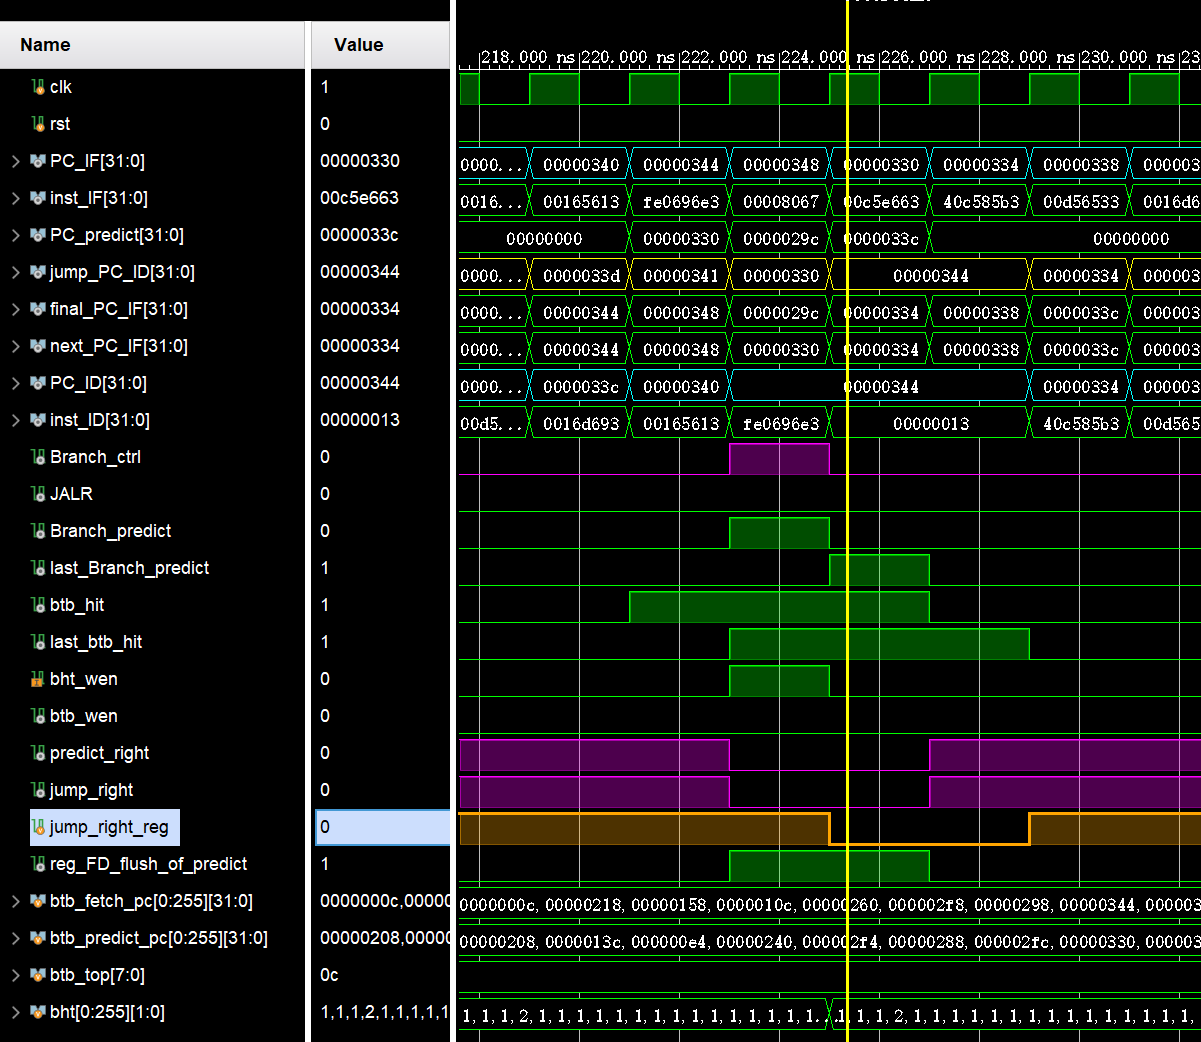
\includegraphics[width=0.8\textwidth]{image/flush_jump_right_reg.png}
            \caption{不考虑 jump\_right\_reg 的 flush 控制}
        \end{figure}

        此时,由于前一个周期预测跳转错误(!jump\_right\_reg),next\_PC\_IF 仍然需要进行跳转为 jump\_PC\_ID;\par
        尽管本周期的预测跳转同样错误(!jump\_right),但错误的预测值 final\_PC\_IF 并没有被写入到 PC\_IF 中;(见1.3 流水线的修改 : 2 next\_PC\_IF的生成)\par
        因而此时不需要对 IF\_ID 寄存器进行 flush 操作。而实际进行了 flush 操作,导致了本应该执行的指令(PC = 0x330)被丢弃。\par
    
        \newpage
        更正后,结果如下:\par
        \begin{figure}[h]
            \centering
            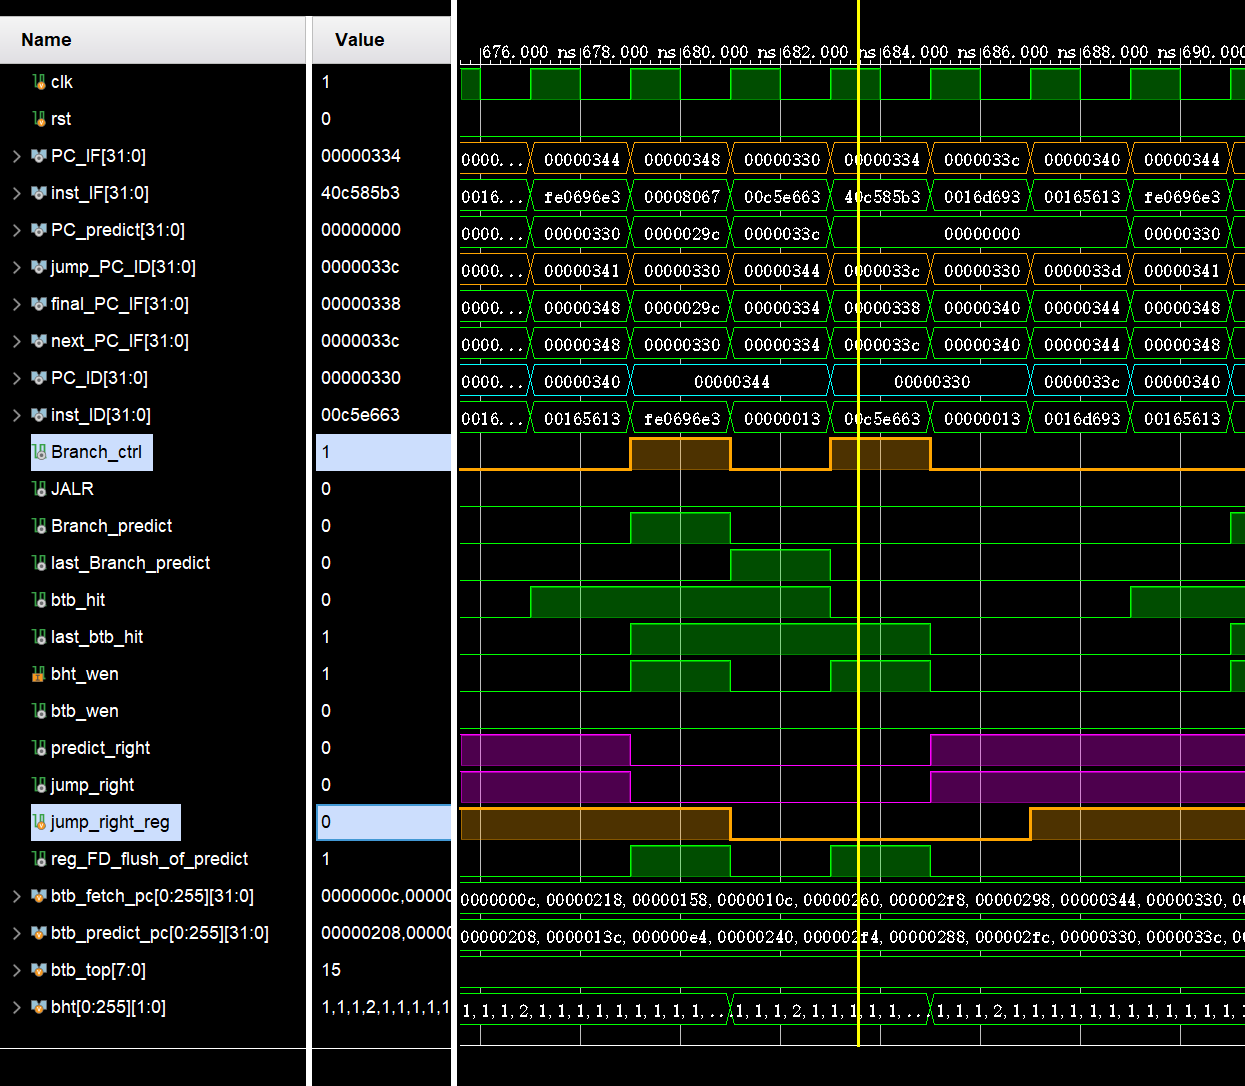
\includegraphics[width=0.8\textwidth]{image/flush_jump_right_reg_fix.png}
            \caption{jump\_right\_reg 问题更正}
        \end{figure}\par
        可见问题已经解决。\par

        \item !jump\_right\_reg 分支下的 Branch\_ctrl 判断:\par 
        在考虑 jump\_right\_reg 为 0 的情况下,还需要考虑 Branch\_ctrl 的值。\par
        若不考虑 Branch\_ctrl 的值:\par
        \begin{lstlisting}[language=Verilog]
    assign reg_FD_flush_of_predict = ~jump_right_reg ? 1'b0 : // jump_right_reg fix
                                            ~jump_right;
        \end{lstlisting}

        \newpage
        则会出现新的问题:\par
        \begin{figure}[h]
            \centering
            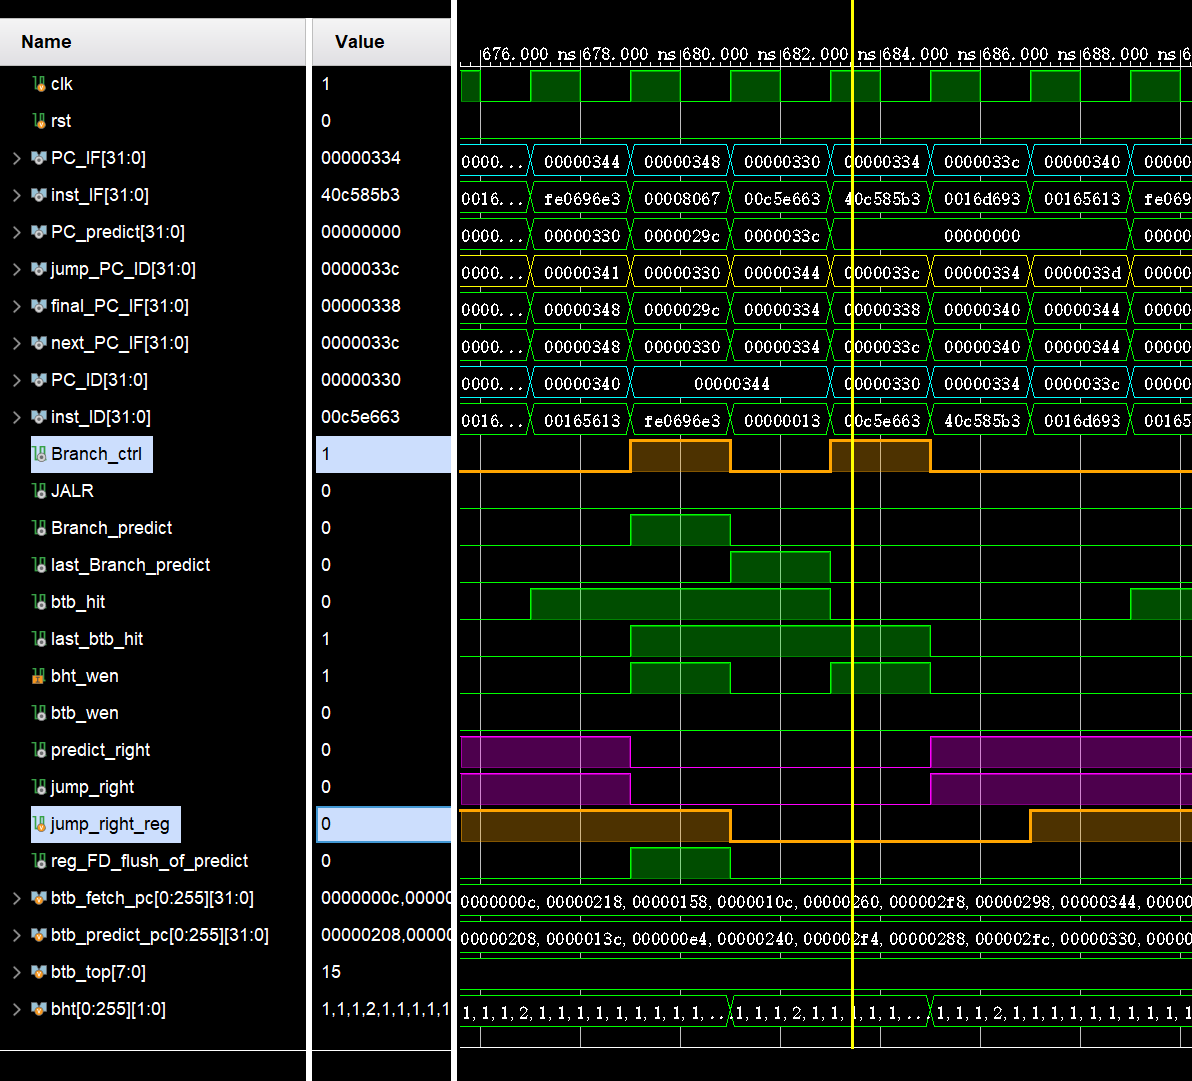
\includegraphics[width=0.8\textwidth]{image/flush_Branch_ctrl.png}
            \caption{jump\_right\_reg 基础上不考虑 Branch\_ctrl 的 flush 控制}
        \end{figure}

        如图 3 所示,当 PC\_IF 为 0x334 时,jump\_right\_reg 信号为 0,然而此时 Branch\_ctrl 信号为 1,
        且 jump\_right 信号为 0,意味着仍需暂停一拍,将错误的 PC\_IF 冲刷掉,这与图中不相符。\par
        因而,当 jump\_right\_reg 信号为 0,且 Branch\_ctrl 信号为 1 时,还需要对 flush 策略进行修正,即:\par
        \begin{lstlisting}[language=verilog]
    assign reg_FD_flush_of_predict = ~jump_right_reg ? Branch_ctrl ? ~jump_right :
                                                                     1'b0;
                                                       ~jump_right;
        \end{lstlisting}

        \newpage
        修正后,结果如下:\par
        \begin{figure}[h]
            \centering
            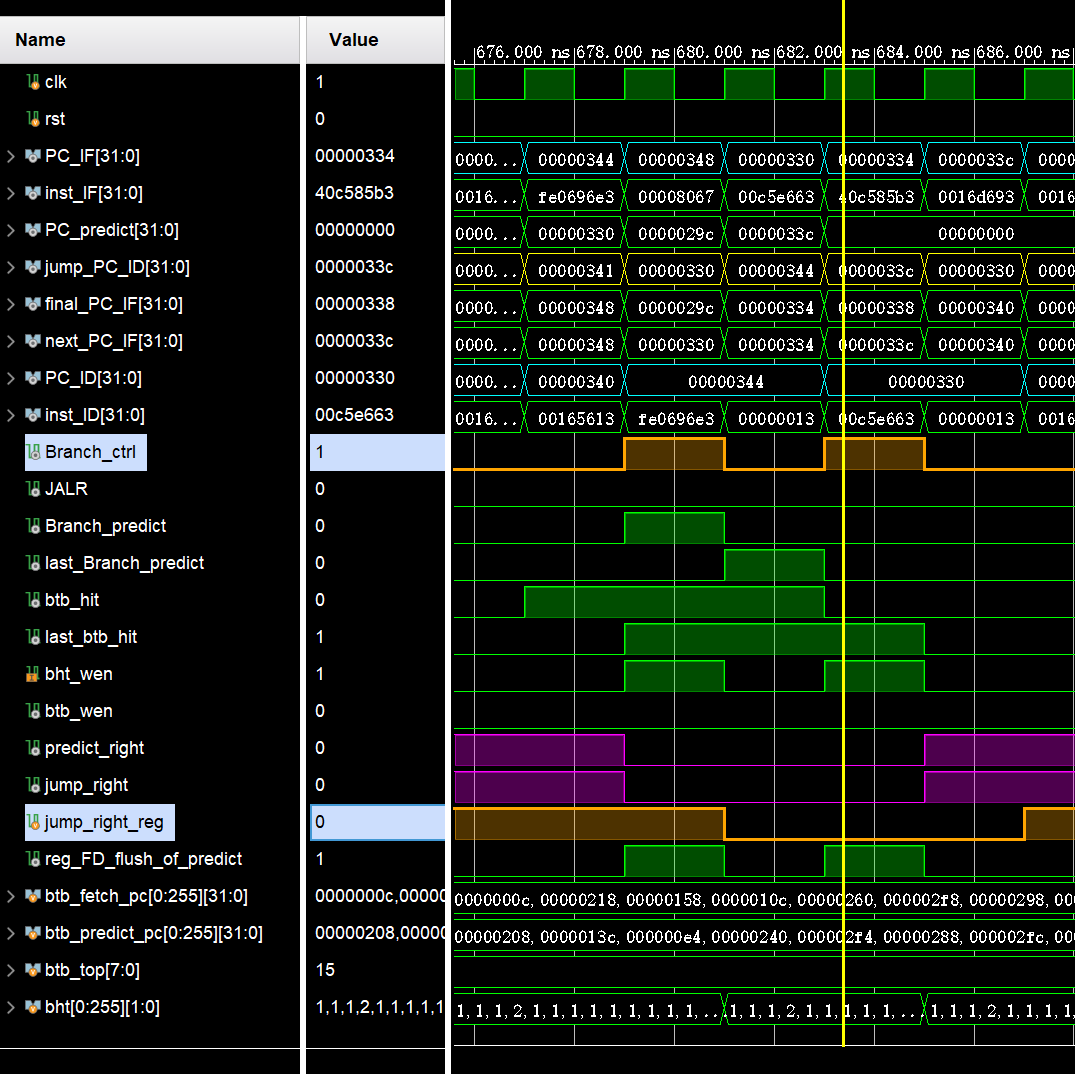
\includegraphics[width=0.8\textwidth]{image/flush_Branch_ctrl_fix.png}
            \caption{考虑 Branch\_ctrl 的 flush 控制}
        \end{figure}

        可见问题已经解决。\par

        \item jump\_right\_reg 问题的延续:\par
        上述对于 jump\_right\_reg 的问题的处理,是对 reg\_FD\_flush\_of\_predict 信号的修正,然而该问题实际上还会影响 jump\_right 等信号的值,进而传递到下一个周期再度引发问题:\par

        \begin{figure}[h]
            \centering
            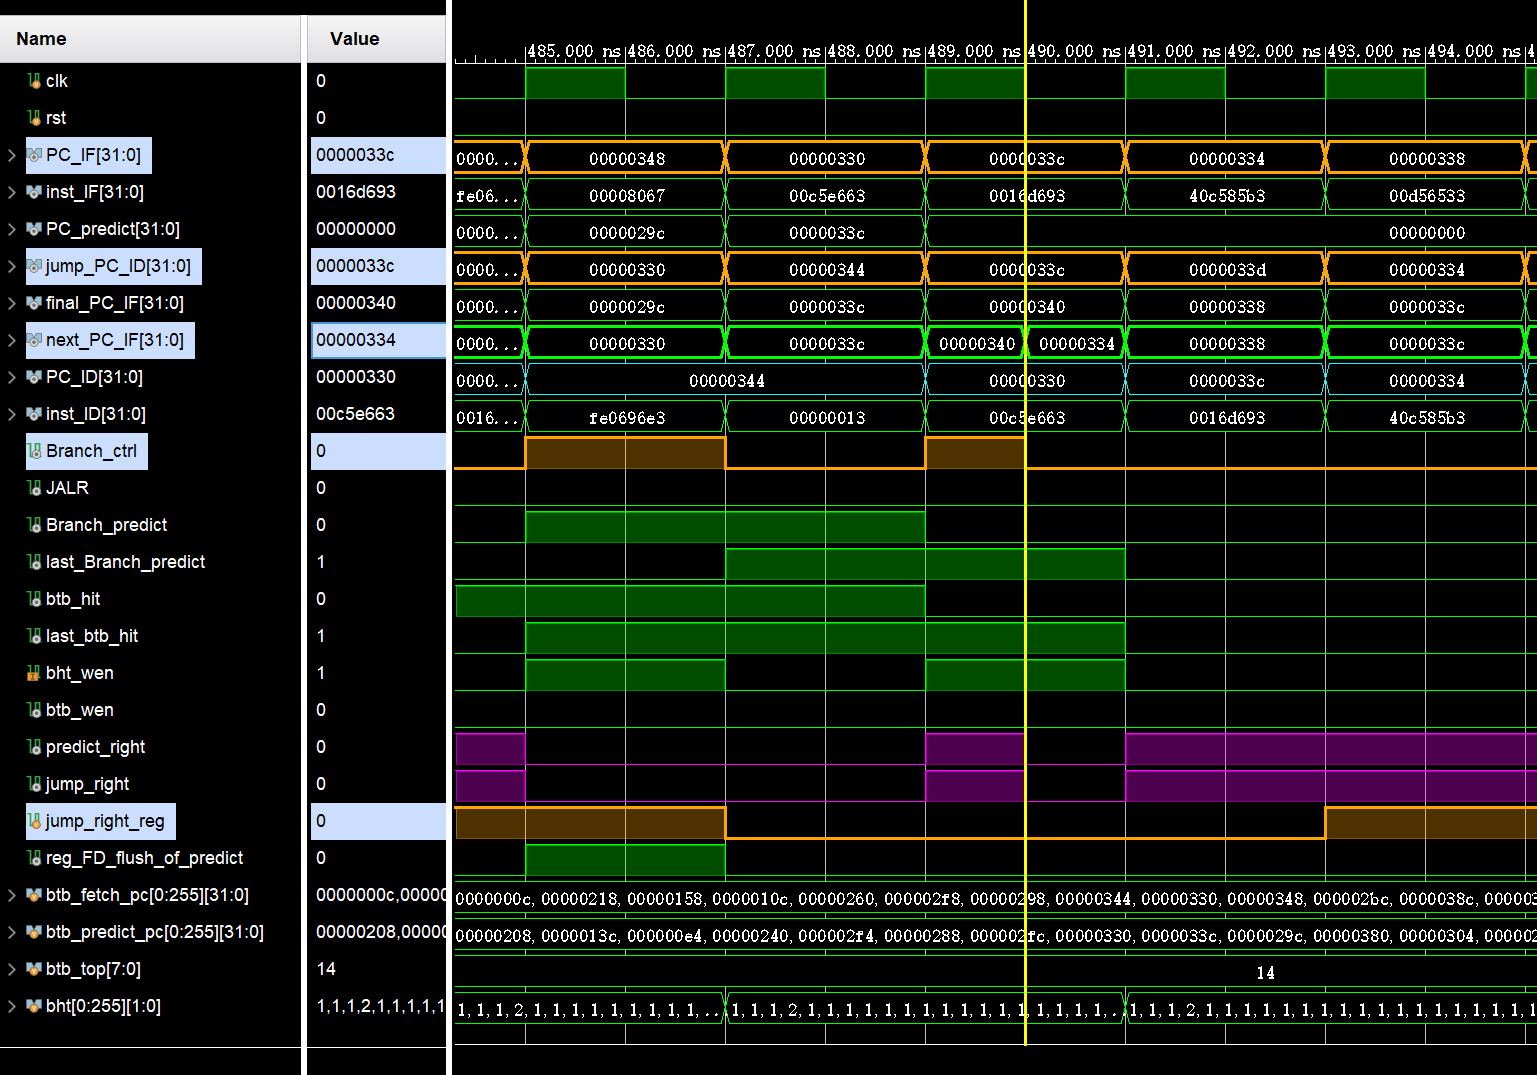
\includegraphics[width=0.8\textwidth]{image/flush_jump_right_reg_reg.png}
            \caption{问题的延续}
        \end{figure}

        \newpage
        (注:由于实现中 Regs 模块采用的是下降沿写入,因而下降沿之后各信号的值才是正确值。)\par
        如图所示,当 PF\_IF 为 0x33c 时,下降沿之后 jump\_right\_reg 信号为 0, 且 Branch\_ctrl 信号为 0,根据之前的修正, reg\_FD\_flush\_of\_predict 信号应当为 0;\par
        然而实际上,PC\_IF = 0x33c 是前一个周期给出的错误预测值,应当被冲刷掉。\par
        这个问题的产生正是因为,前一个周期的 jump\_right\_reg 信号也为 0,虽然该周期对 reg\_FD\_flush\_of\_predict 信号进行了正确修正,但该周期的 jump\_right 信号其实是错误的,且被传递到了下一个周期。\par
        
        因此,仍需要添加补丁,如下:\par
        \begin{lstlisting}[language=Verilog]
    assign reg_FD_flush_of_predict = ~jump_right_reg ? Branch_ctrl ? ~jump_right : 
                                                PC_IF == jump_PC_ID : // jump right
                                            ~jump_right; // jump when no branch
        \end{lstlisting}

        \newpage
        修正后,结果如下:\par
        \begin{figure}[h]
            \centering
            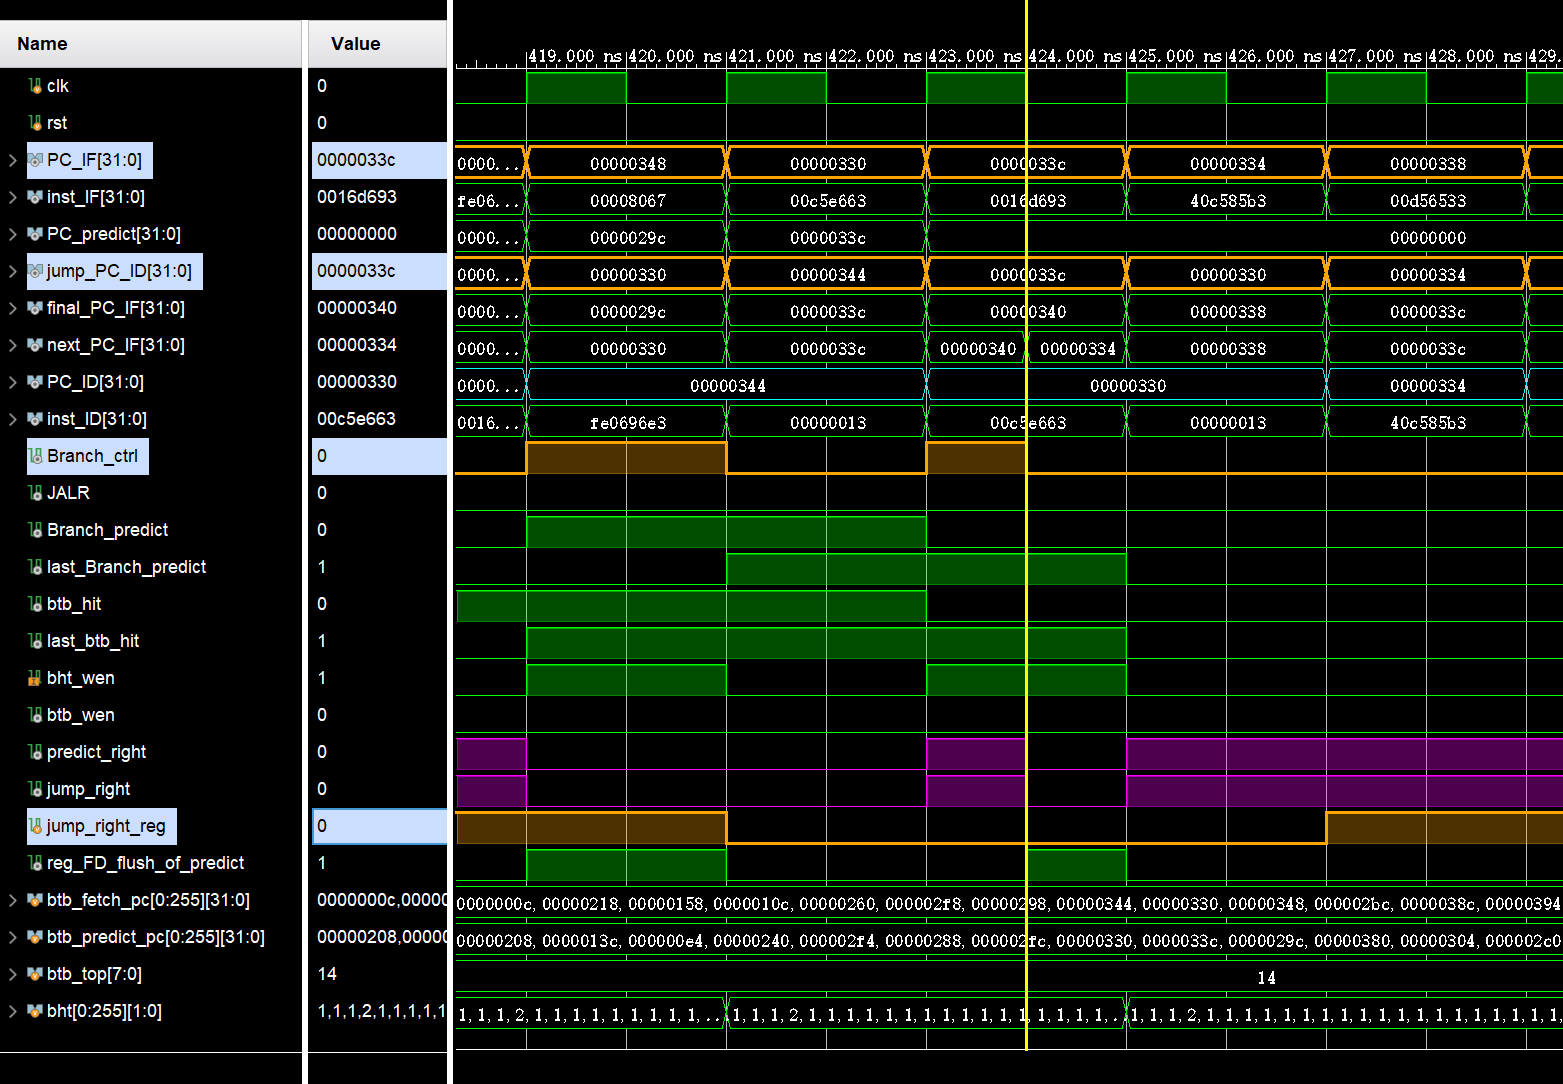
\includegraphics[width=0.8\textwidth]{image/flush_jump_right_reg_reg_fix.png}
            \caption{问题的延续修正}
        \end{figure}
        可见问题已经解决。\par
    \end{enumerate}
\end{enumerate}


\newpage
\section{仿真结果与上板验证}
    \begin{enumerate}
        \item 仿真结果如下:\par
        \begin{figure}[h]
            \centering
            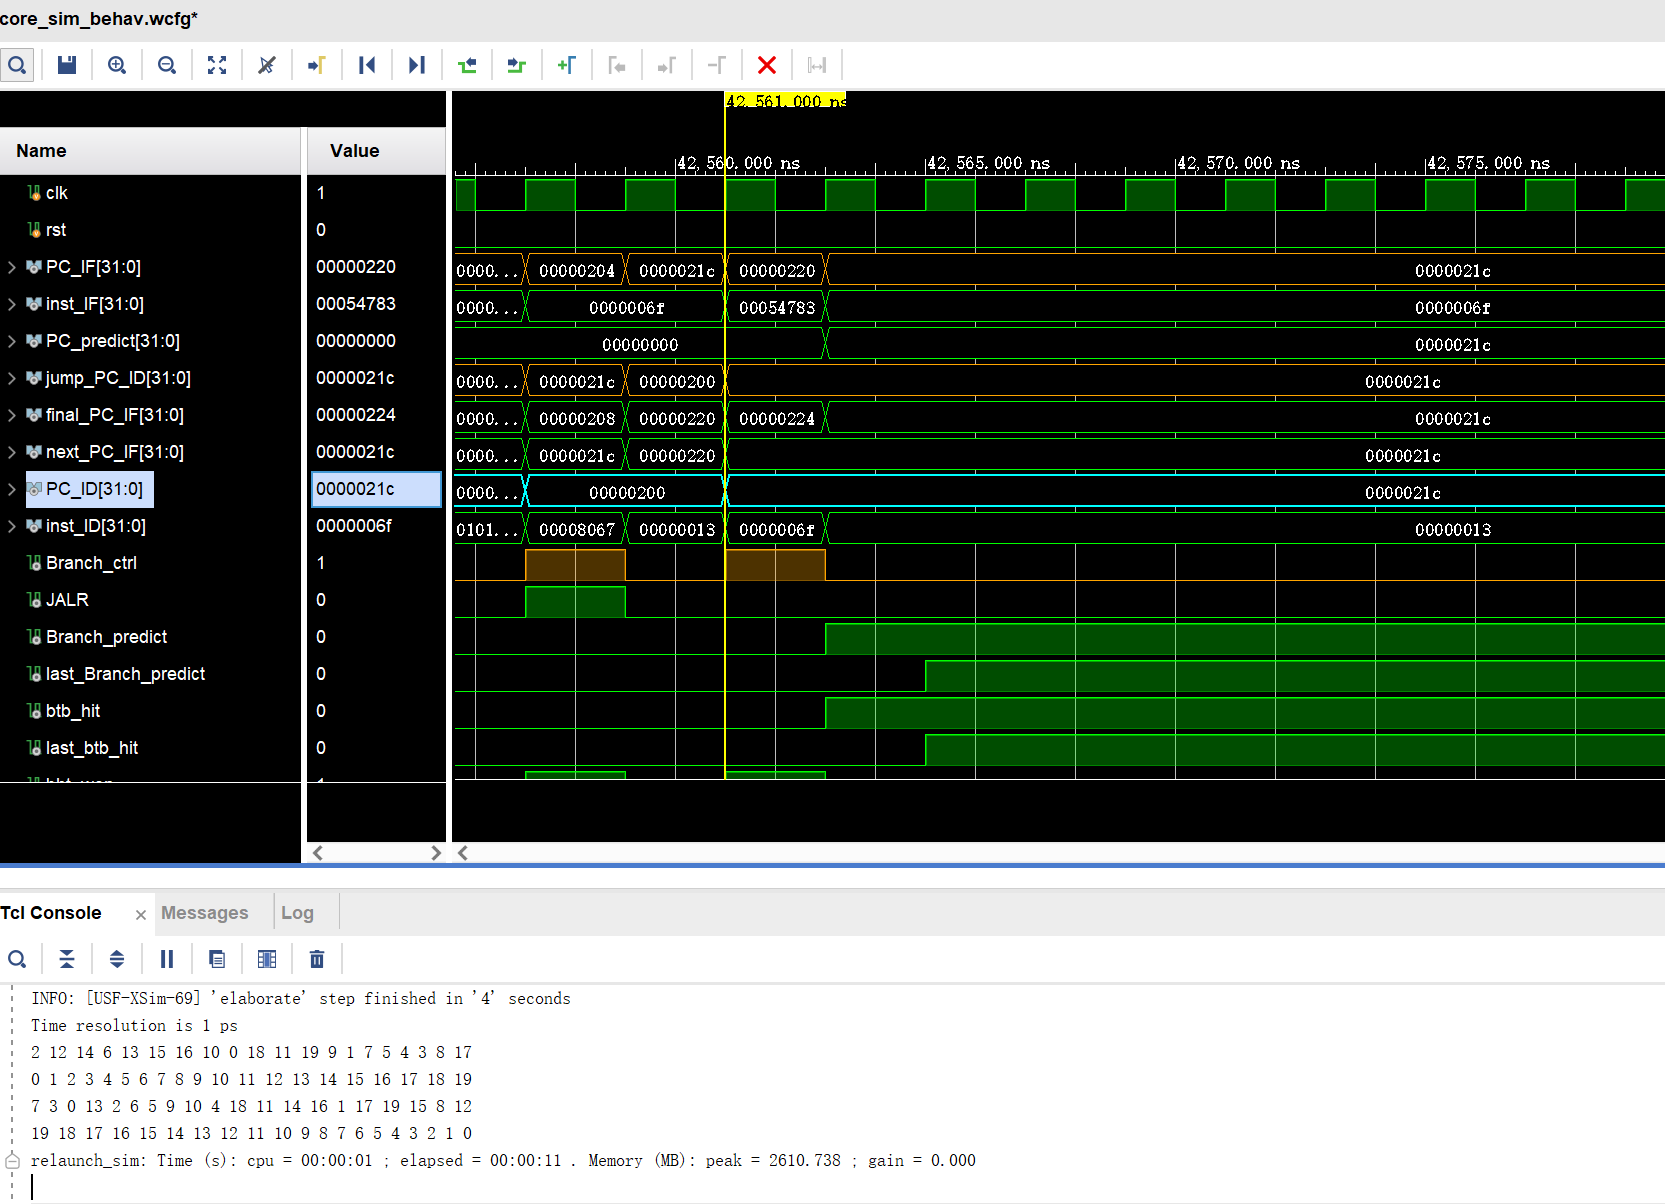
\includegraphics[width=0.8\textwidth]{image/sim.png}
            \caption{仿真结果}
        \end{figure}
        可见,仿真正确输入了预期值,且仿真进入循环的时间为 42561 ns,达到了实验要求的阈值。\par
        实验设计符合预期。\par

        \item 上板验证结果如下:\par
        \begin{figure}[h]
            \centering
            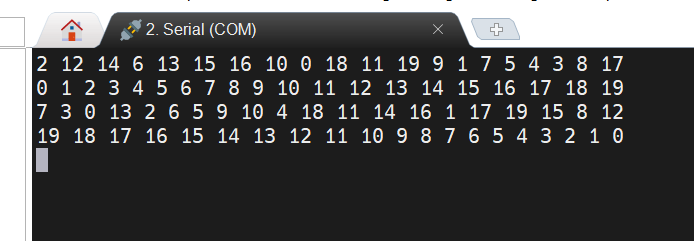
\includegraphics[width=0.8\textwidth]{image/board.png}
            \caption{上板验证结果}
        \end{figure}
        可见,上板验证时串口输出值正确,实验设计符合预期。\paragraph[short]{title}

    \end{enumerate}

\section{思考题 1}
\begin{enumerate}
    \item \textbf{加了分支预测后,仿真跑测试程序,较没加的时候快了多少?以仿真中进入 loop 的时间作为程序运行时间,计算加速比。}\par
    未添加分支预测时,仿真结果如下:\par
    \begin{figure}[h]
        \centering
        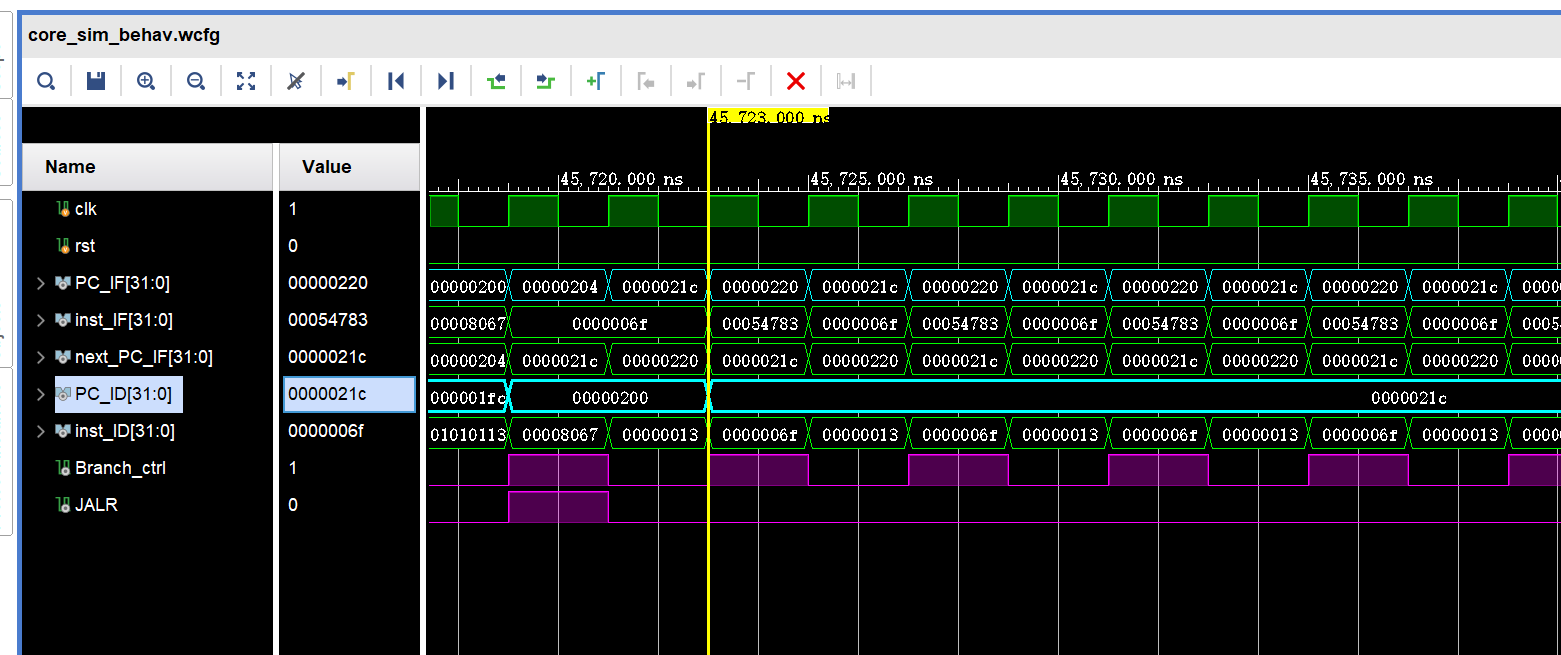
\includegraphics[width=0.8\textwidth]{image/sim_no_prediction.png}
        \caption{未添加分支预测时的仿真结果}
    \end{figure}
    可见此时进入循环的仿真时间为 45732 ns。\par
    与我添加预测后的仿真时间 42561 ns 相比,速度提升了 6.93\%。\par

    \newpage
    \item \textbf{请在报告里展示以下五种仿真波形:}\par
    \begin{itemize}
        \item 分支预测跳转,实际不跳转,分支预测不跳转,实际跳转\par
        \begin{figure}[h]
            \centering
            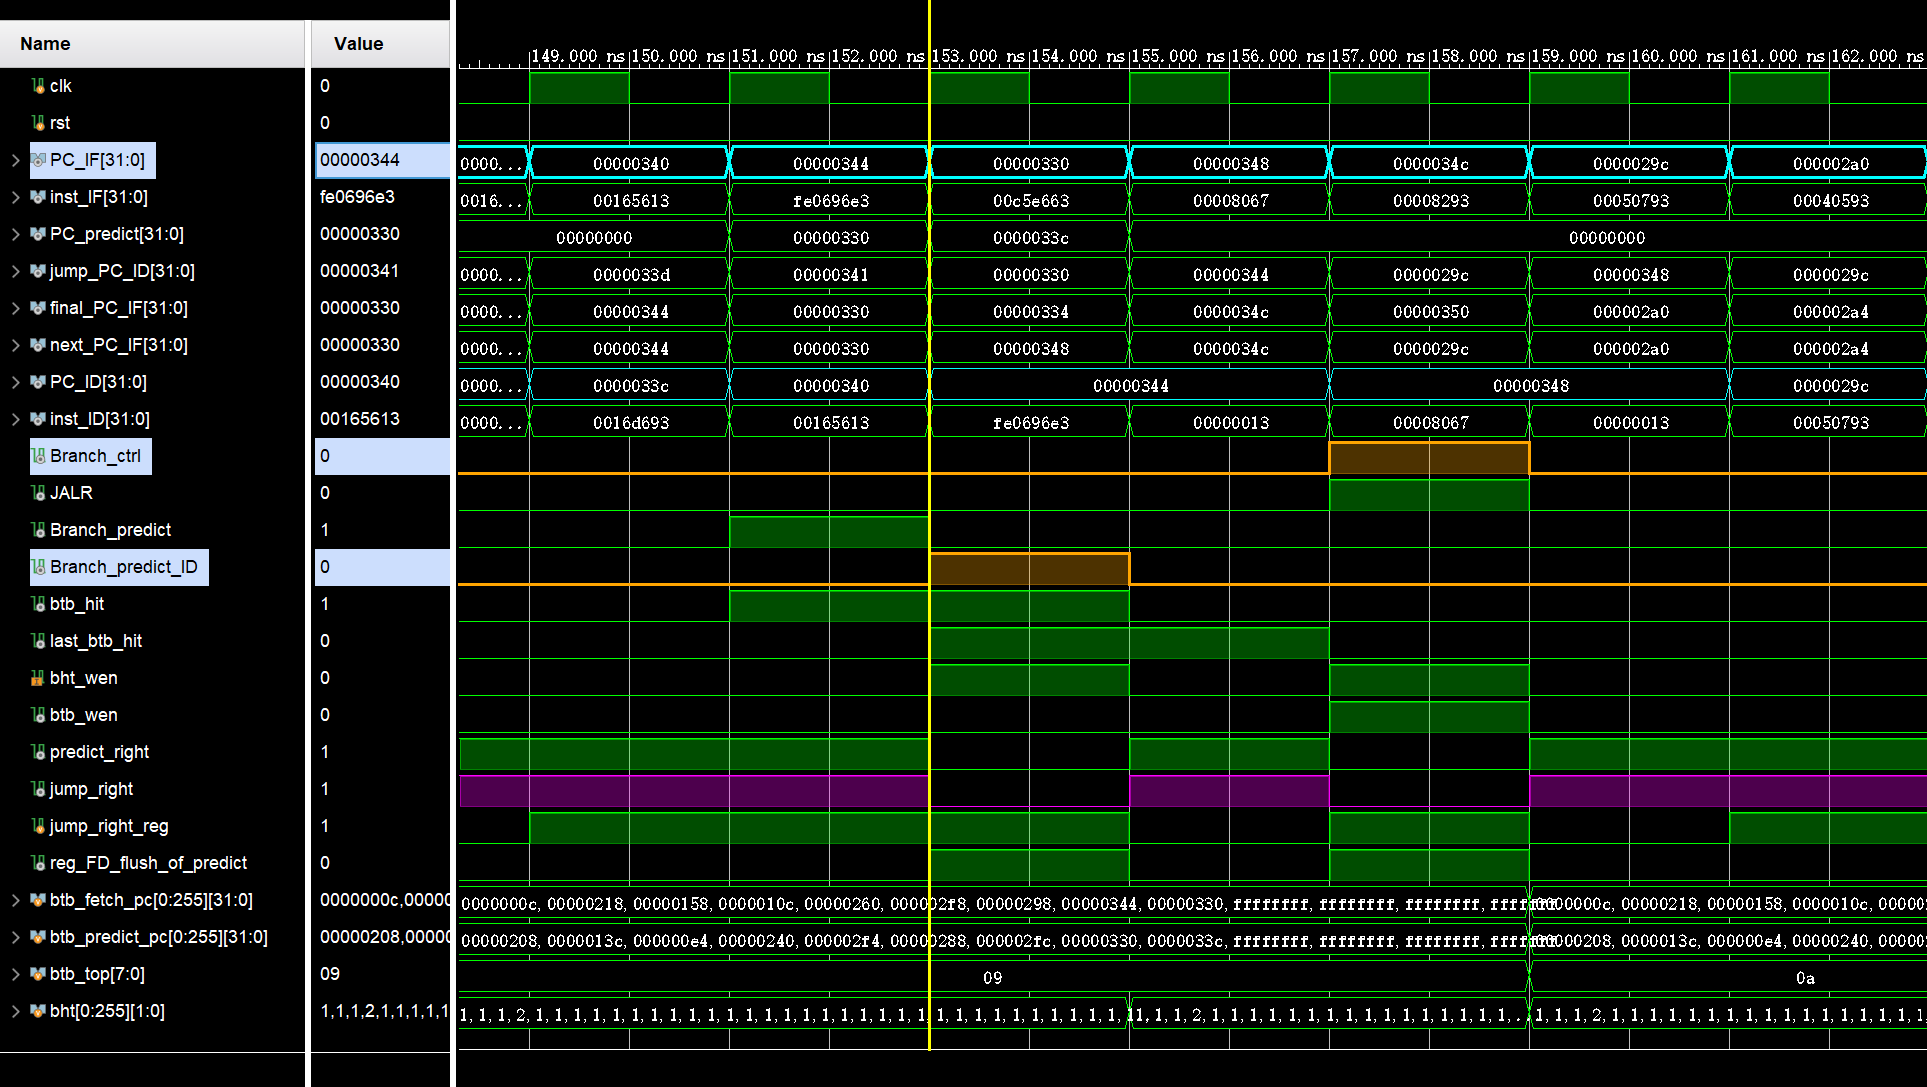
\includegraphics[width=0.8\textwidth]{image/thinking2_fig1.png}
            \caption{分支预测跳转,实际不跳转 以及 分支预测不跳转,实际跳转}
        \end{figure}
        如图,PC\_IF = 0x34c 时,即为分支预测跳转,实际不跳转的情形。\par
        而 PC\_IF = 0x330 时,即为分支预测不跳转,实际跳转的情形。\par

        \newpage
        \item 分支预测跳转,实际跳转,BTB 给出的跳转地址正确\par
        \begin{figure}[h]
            \centering
            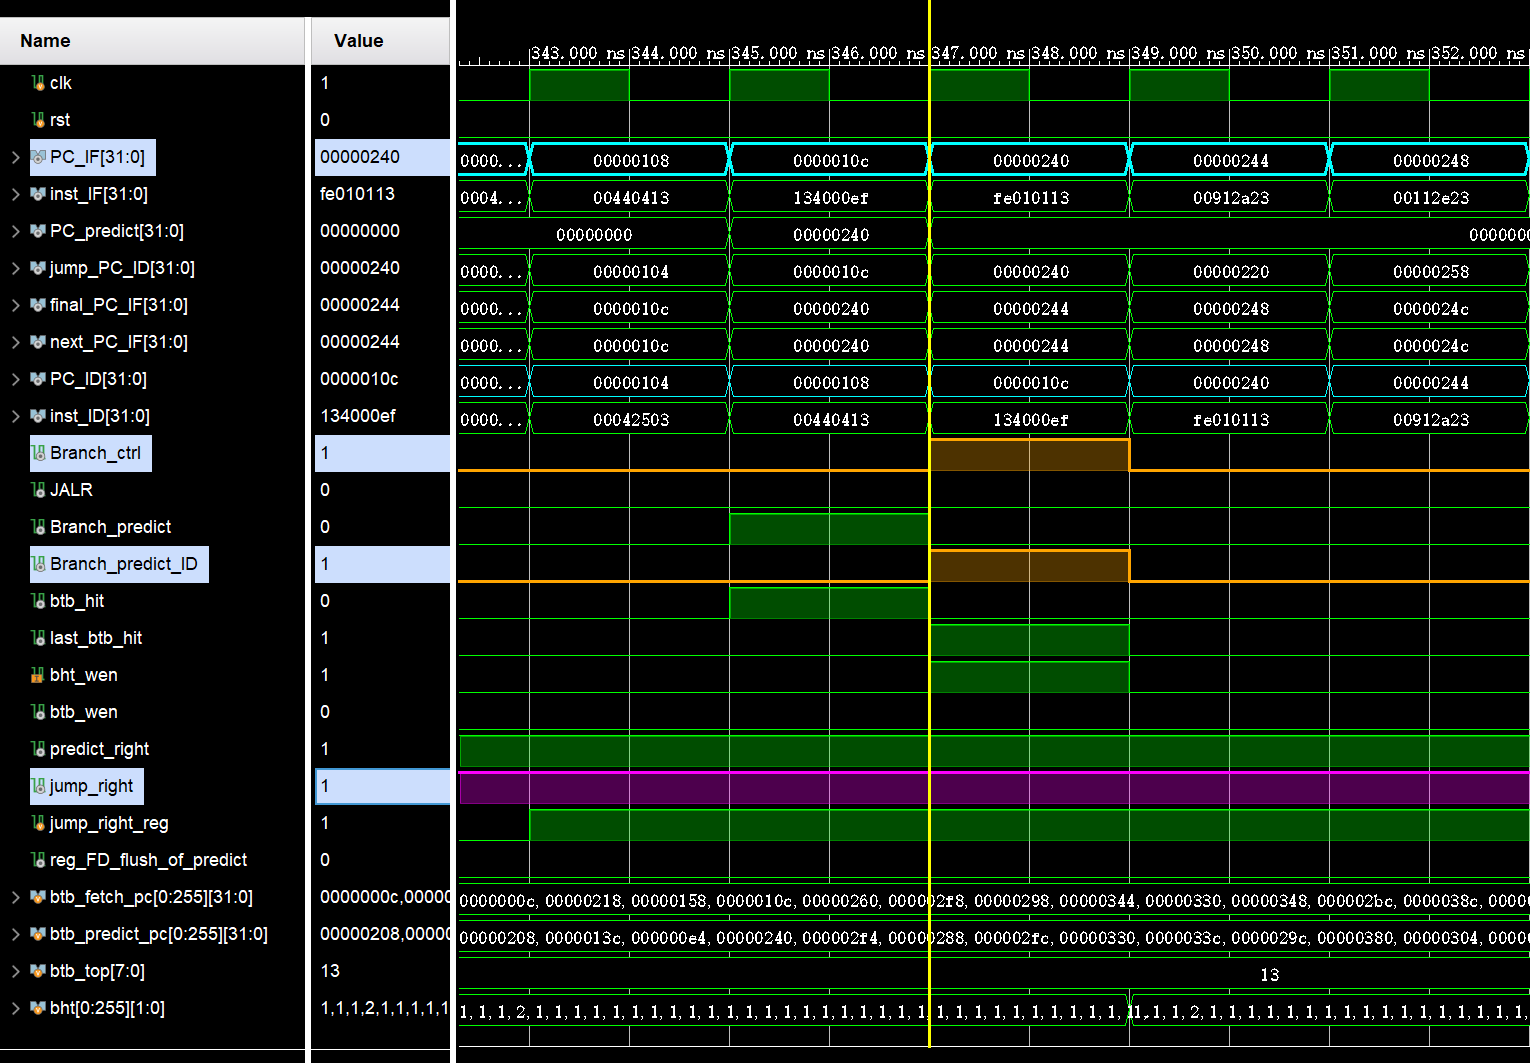
\includegraphics[width=0.8\textwidth]{image/thinking2_fig2.png}
            \caption{分支预测跳转,实际跳转,BTB 给出的跳转地址正确}
        \end{figure}
        如图,PC\_IF = 0x240 时,即为分支预测跳转,实际跳转,BTB 给出的跳转地址正确的情形。\par

        \newpage
        \item 分支预测跳转,实际跳转,BTB 给出的跳转地址错误\par
        \begin{figure}[h]
            \centering
            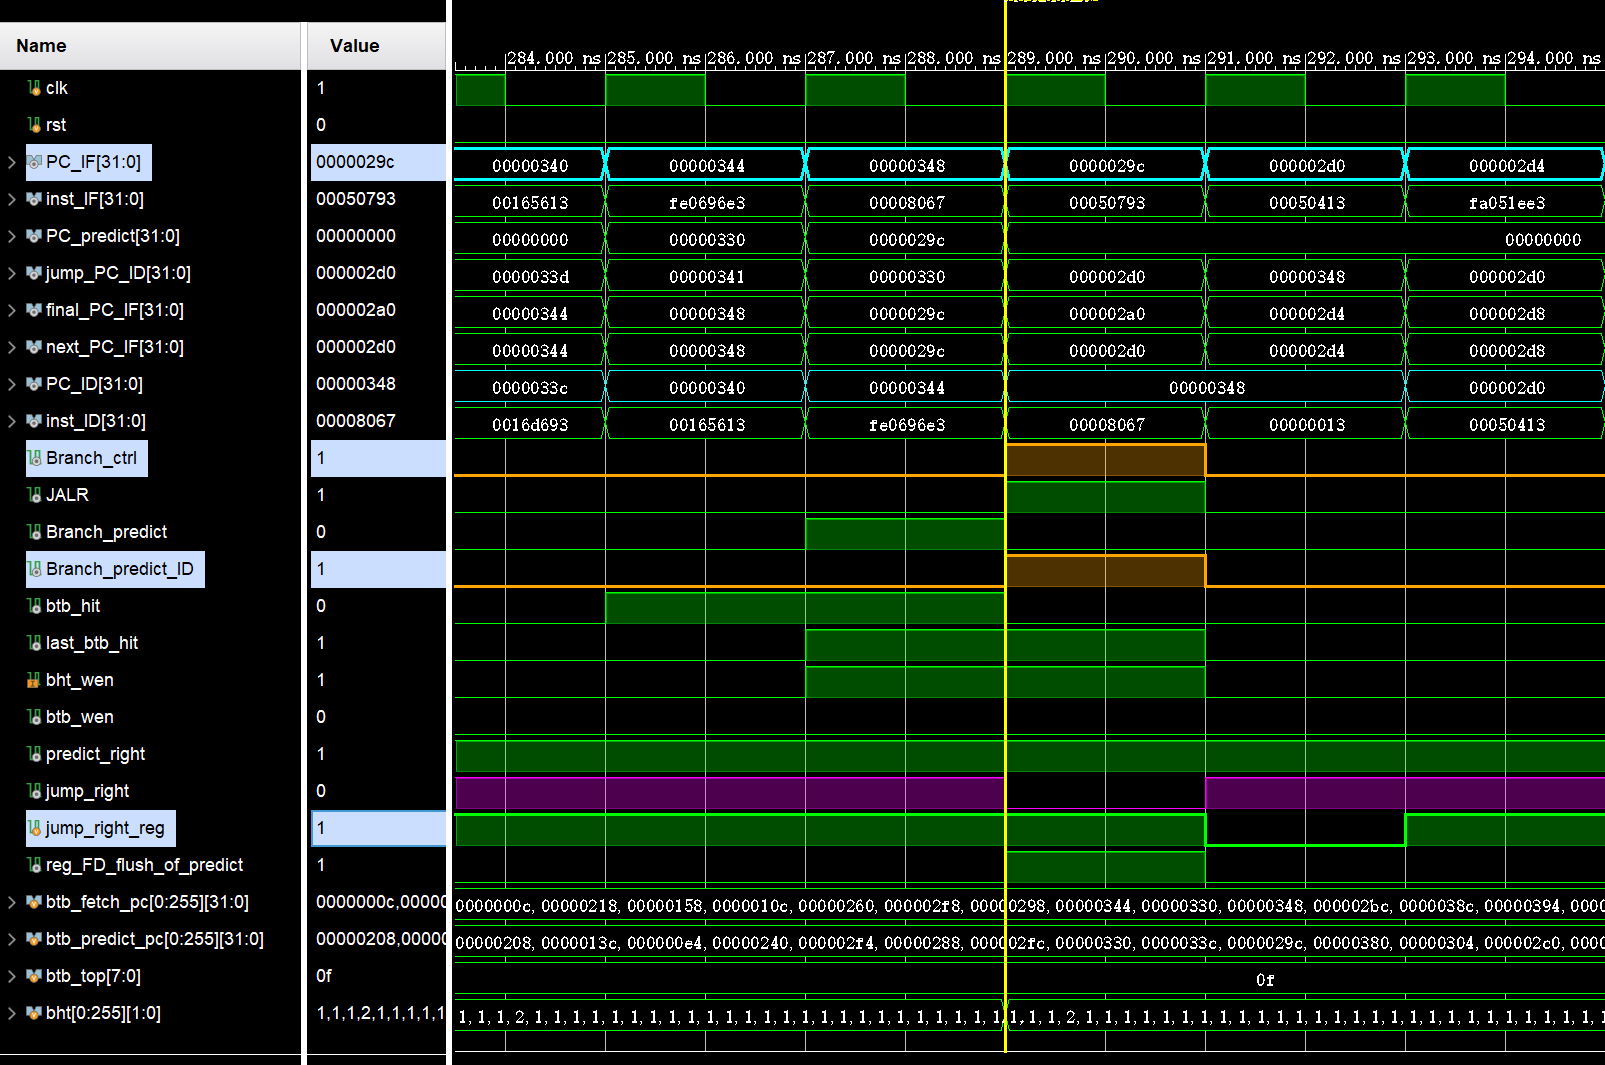
\includegraphics[width=0.8\textwidth]{image/thinking2_fig3.png}
            \caption{分支预测跳转,实际跳转,BTB 给出的跳转地址错误}
        \end{figure}
        如图,PC\_IF = 0x297 时,即为分支预测跳转,实际跳转,BTB 给出的跳转地址错误的情形。\par
        
        \newpage
        \item 分支预测不跳转,实际不跳转\par
        \begin{figure}[h]
            \centering
            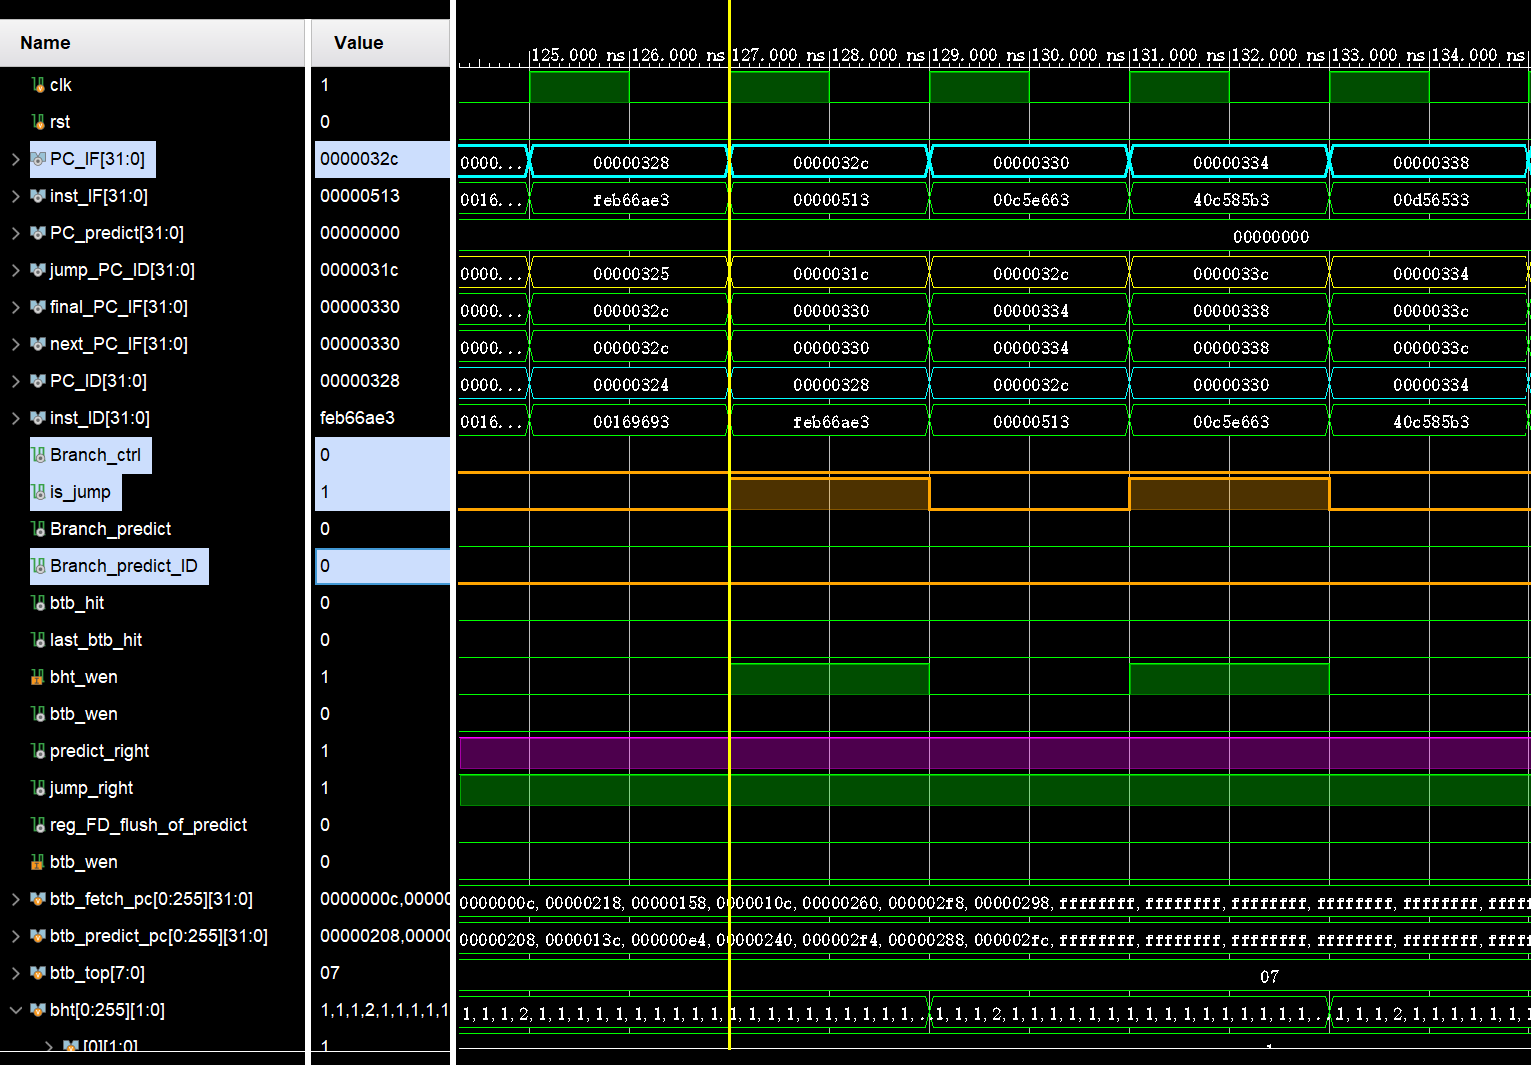
\includegraphics[width=0.8\textwidth]{image/thinking2_fig4.png}
            \caption{分支预测不跳转,实际不跳转}
        \end{figure}
        如图,PC\_IF = 0x32c 与 0x332 时,均为分支预测不跳转,实际不跳转的情形。\par
    \end{itemize}
    
    \item \textbf{相比于静态分支预测,说明动态分支预测的优点以及缺点。}\par
    \begin{itemize}
        \item 优点:\par
        动态分支预测处理复杂分支模式,对嵌套循环、条件依赖型分支(如 if-else 链)的预测能力更强,拥有更高的预测准确率,能够较大程度地减少跳转指令在流水线中的延迟,加速流水线。
        \item 缺点:\par
        \begin{enumerate}
            \item 存储开销增大,需维护BHT、BTB等结构,典型设计占用数KB至数十KB存储;\par
            \item 预测逻辑需在取指阶段前完成,可能限制时钟频率提升。
            \item 在某些特定情况下,如程序较小时或特定循环情况下,误预测可能较多,冲刷后续指令可能带给流水线较大代价。
        \end{enumerate}
    \end{itemize}


\end{enumerate}


\end{document}